\begin{figure}[htp]
\centering
\subfloat[a]{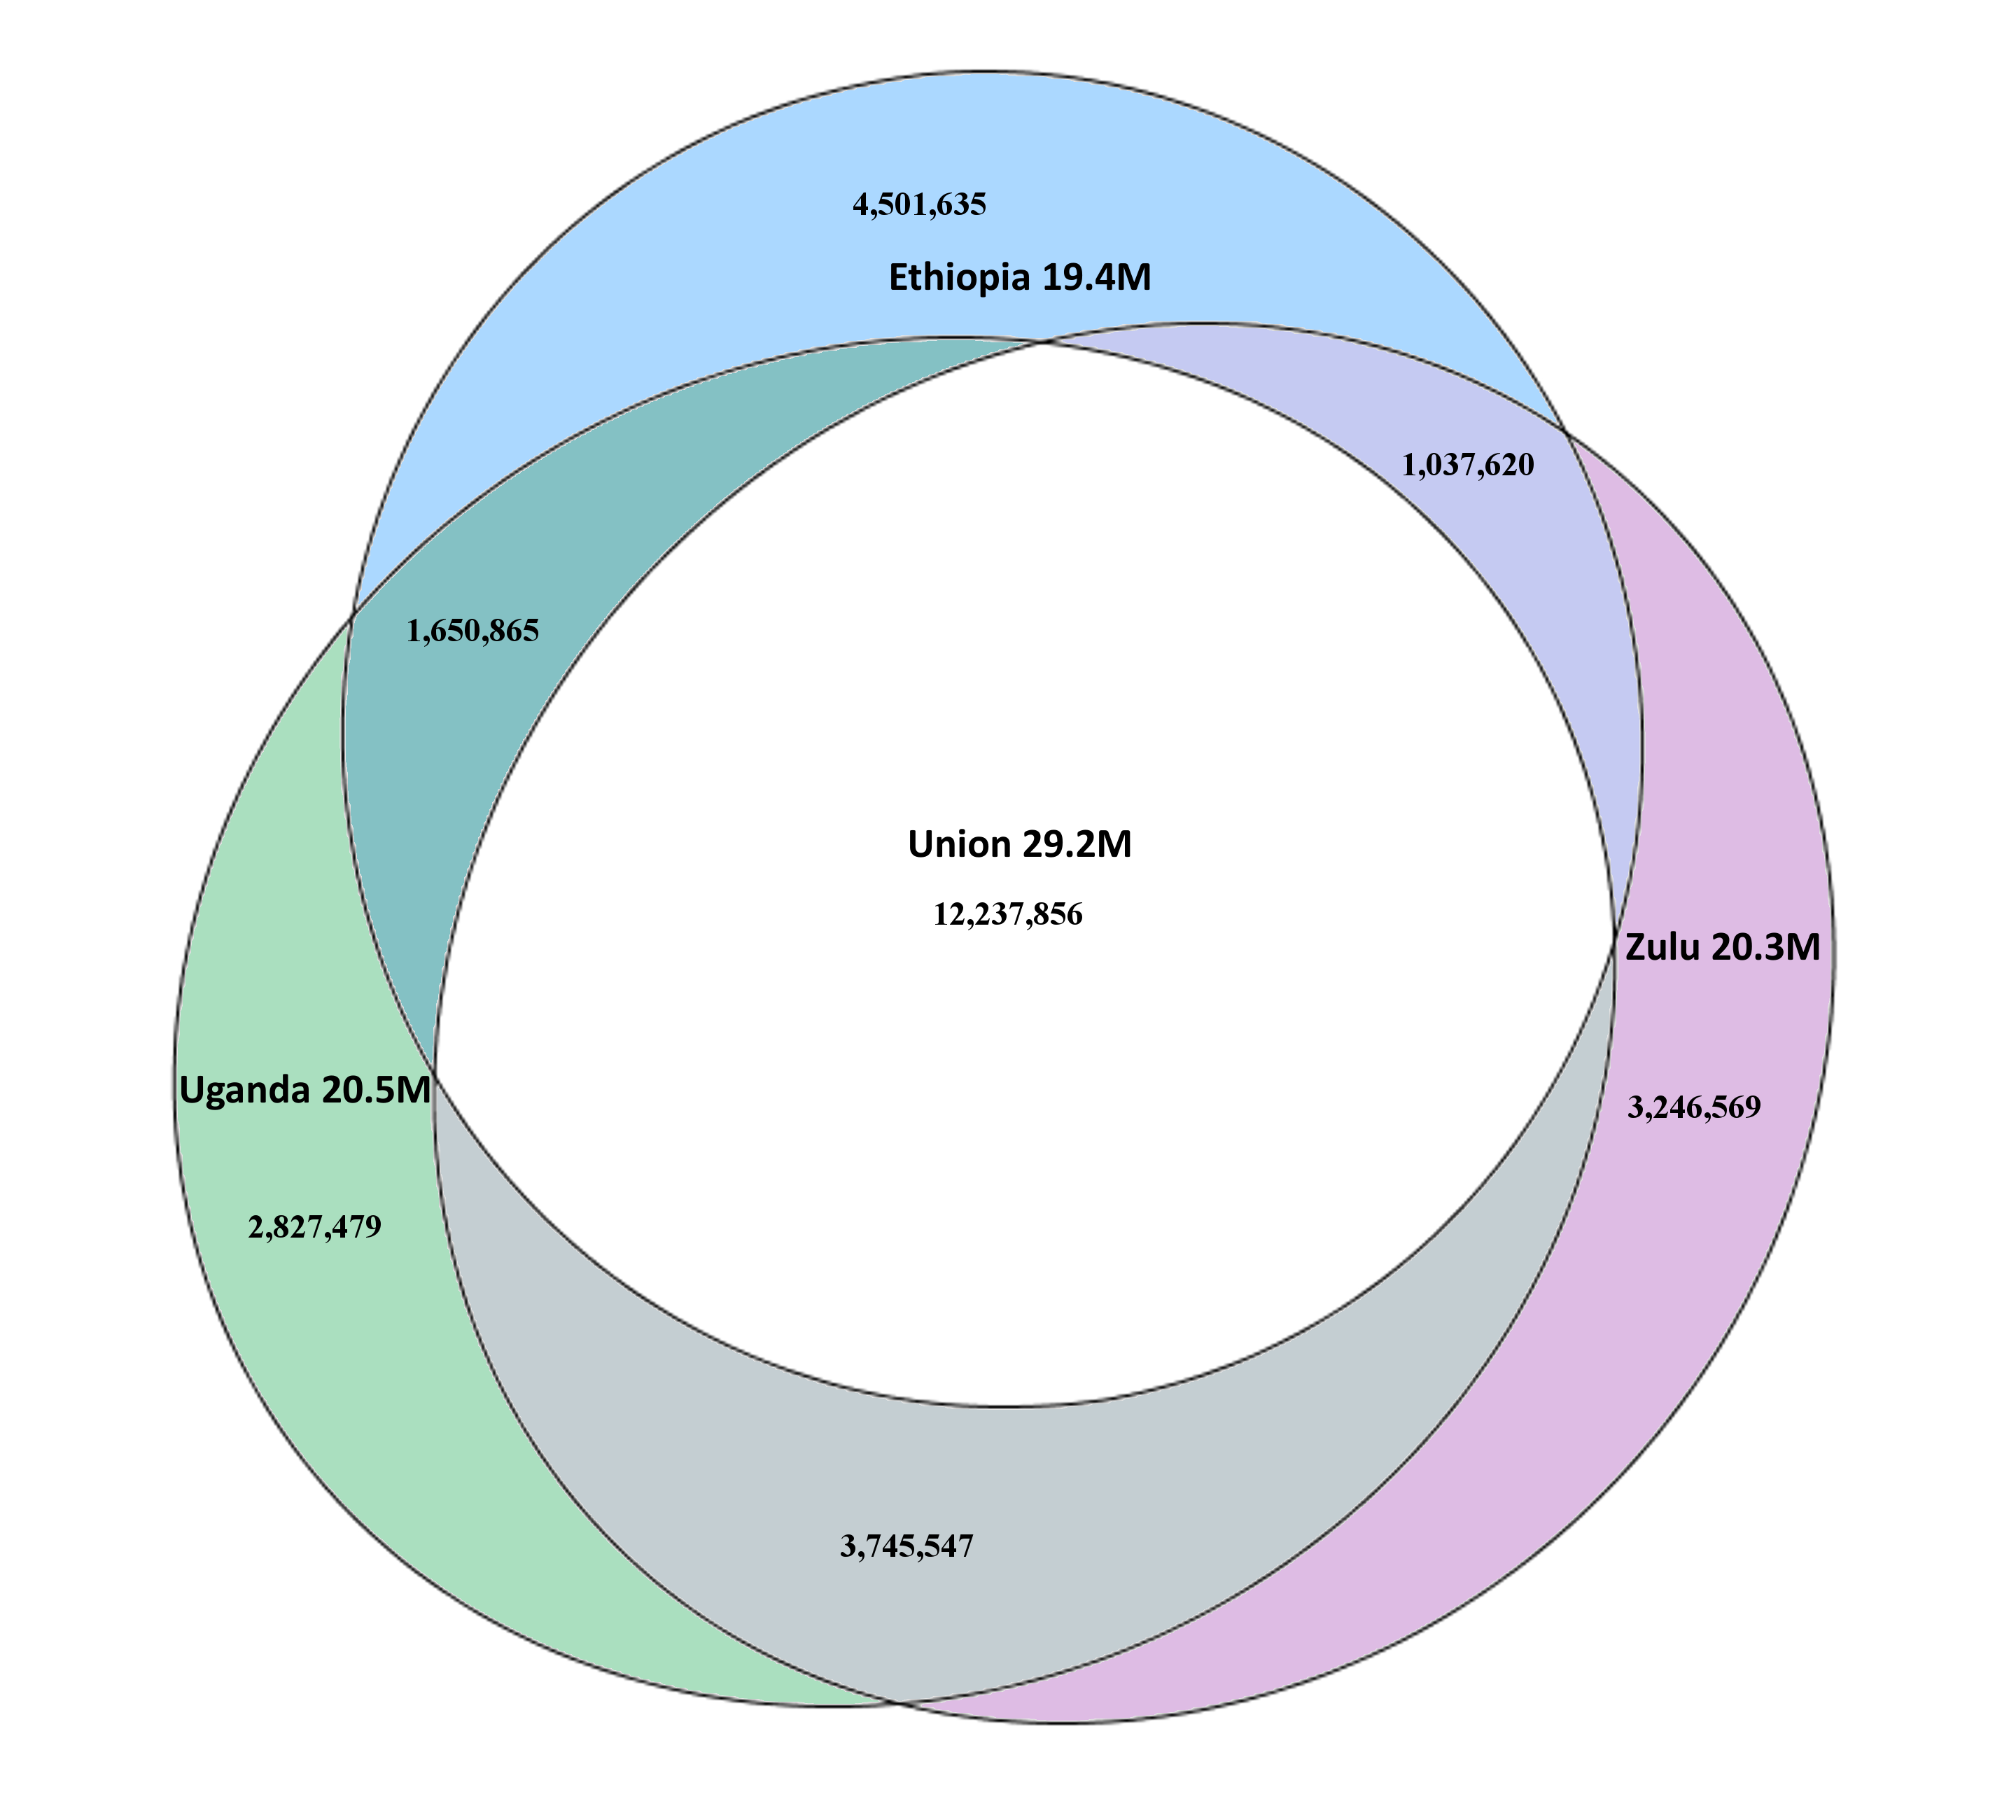
\includegraphics[width=0.4\linewidth]{Chapter2/fig/venn3.png}}
\subfloat[b]{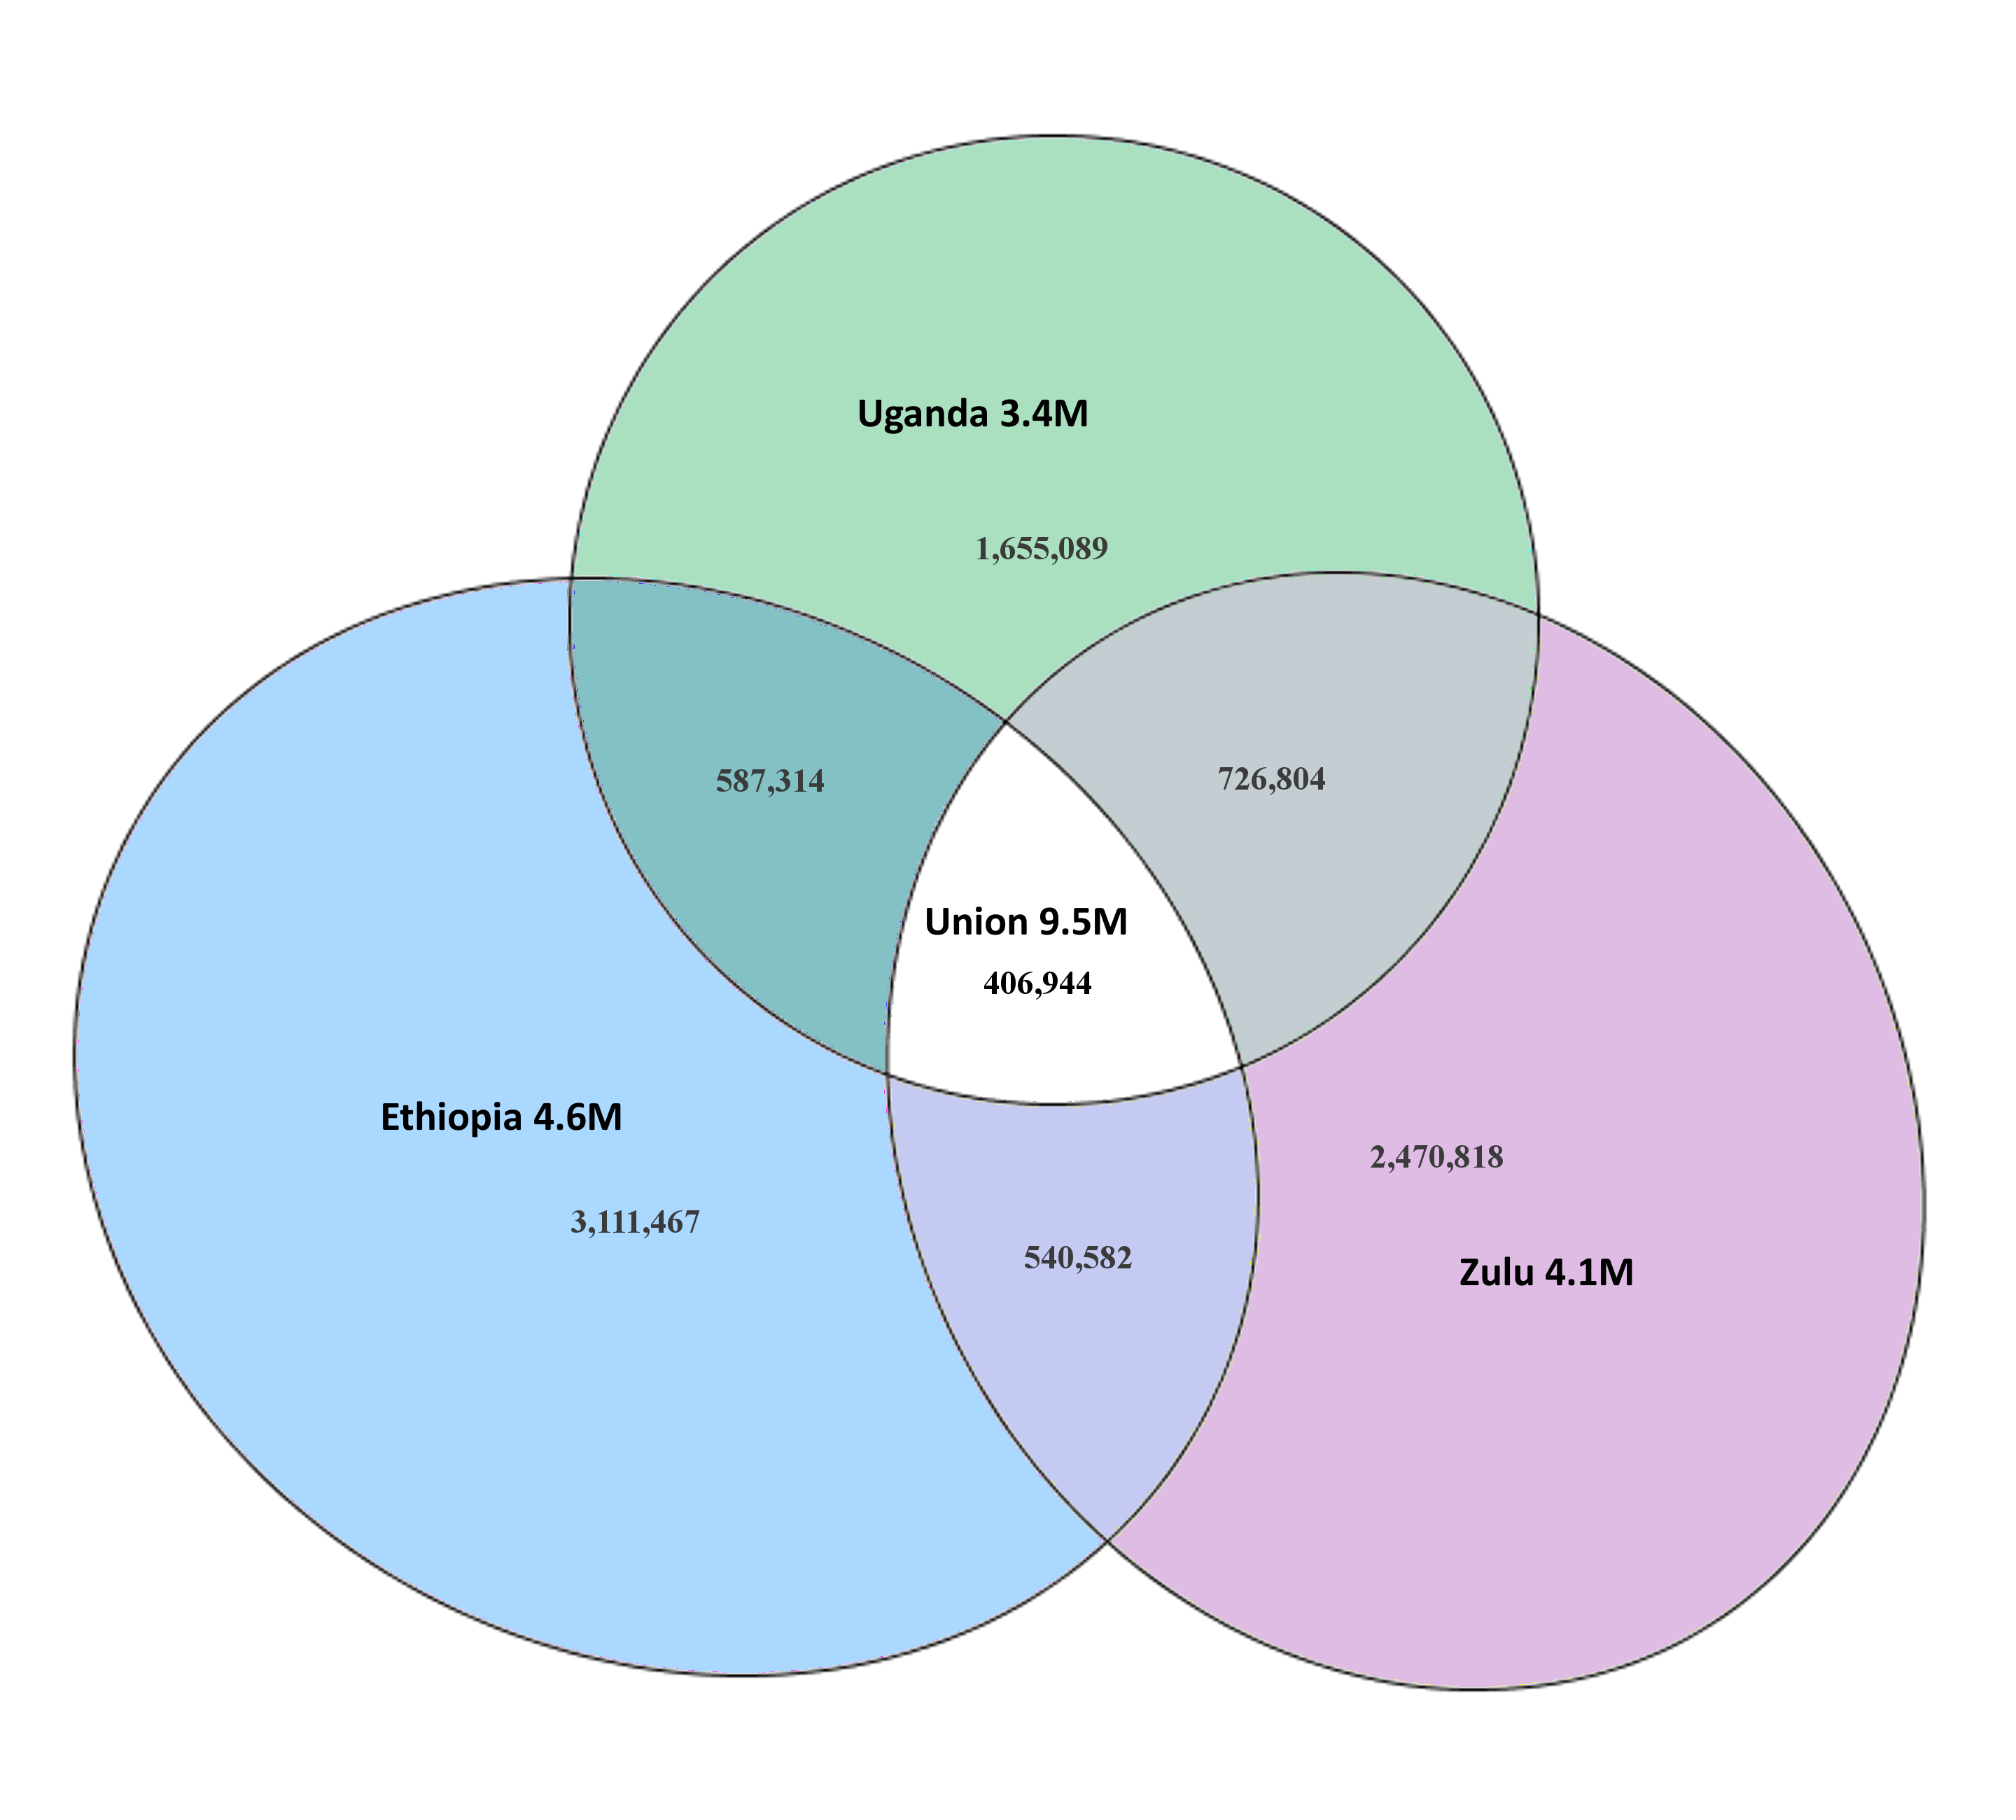
\includegraphics[width=0.4\linewidth]{Chapter2/fig/venn3_complement.png}}
\subfloat[c]{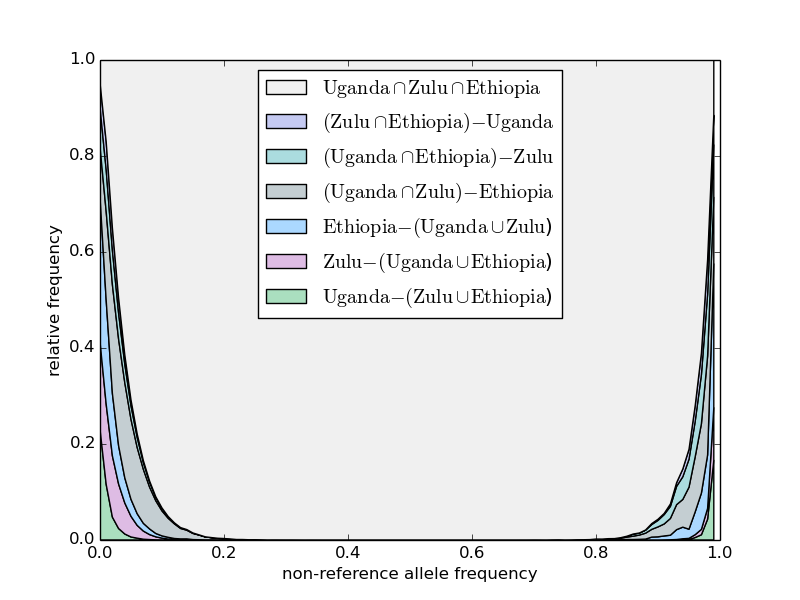
\includegraphics[width=0.4\linewidth]{Chapter2/fig/venn3_stackplot_SNPs.png}}
\subfloat[d]{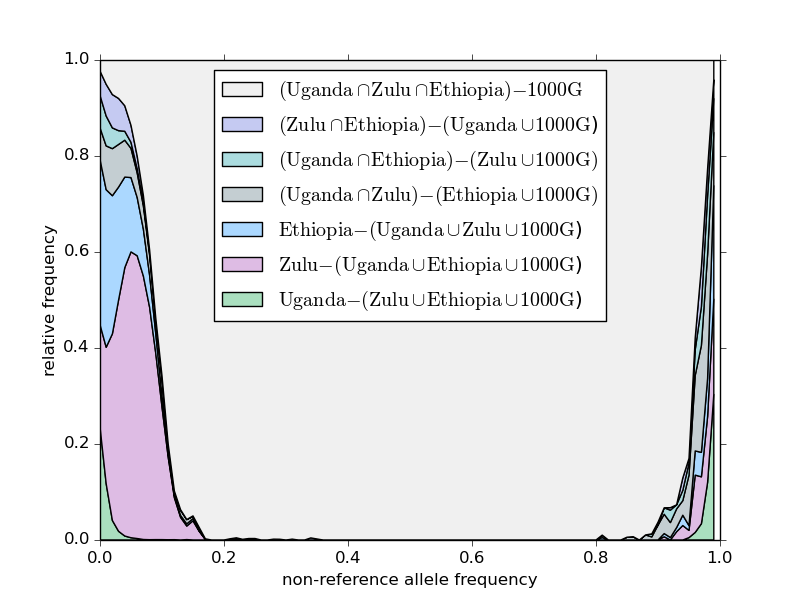
\includegraphics[width=0.4\linewidth]{Chapter2/fig/venn3_stackplot_complement_1000G_SNPs.png}} 
\caption{Sharing of variants between populations. a) SNP intersection between the 3 sequenced populations subsampled to 100 samples and downsampled to 4x coverage. b) Intersection between the novel variants in the 3 populations; i.e. variants in the relative complement of \gls{1000G} phase 1 with respect to the 3 populations. c) Relative allele frequency spectra for variants in different sets of the Venn diagrams depicted in a and b. The majority of the novel variants with respect to \gls{1000G} are unique to each population. Figures were created with eulerAPE\cite{10.1371/journal.pone.0101717} and matplotlib\cite{Hunter2007}}
\label{fig:intersection}
\end{figure}